\documentclass[xetex,18pt,aspectratio=43]{beamer}

\usepackage{caption}
\usepackage[percent]{overpic}
\usepackage{xecyr}
\usepackage{xunicode}
\usepackage[absolute,overlay]{textpos}
\usepackage{fontspec}
\usepackage{calc}
\usepackage{multicol}
\usepackage{hyperref}
\usepackage{setspace}
\usepackage{tikz}
%\usepackage[texcoord,grid,gridunit=mm,gridcolor=red!10,subgridcolor=green!10]{eso-pic}
\defaultfontfeatures{Ligatures=TeX}
\setmainfont{Trebuchet MS}
\usepackage{polyglossia}
\setdefaultlanguage[spelling=modern]{russian}
\newfontfamily{\cyrillicfont}{Trebuchet MS}
\newfontfamily{\cyrillicfontsf}{Trebuchet MS}
\newfontfamily{\cyrillicfonttt}{Trebuchet MS}

\newcommand\Bigfont{\fontsize{22}{22}\selectfont}
\newcommand\Authorfont{\fontsize{17}{17}\selectfont}
\newcommand\Orgfont{\fontsize{13}{13}\selectfont}

\mode<presentation>
{
  %\usetheme{Boadilla}      % or try Darmstadt, Madrid, Warsaw, ...
  \usecolortheme{default} % or try albatross, beaver, crane, ...
  %\usefonttheme{default}  % or try serif, structurebold, ...
  \setbeamertemplate{navigation symbols}{}
  \setbeamertemplate{caption}[numbered]
  \setbeamertemplate{itemize items}[circle]
  \setbeamerfont{title}{series=\bfseries,parent=structure}
  \setbeamerfont{frametitle}{size=\huge}
} 

\makeatother
\setbeamertemplate{footline}
{
  \leavevmode%
  \hbox{%
  \begin{beamercolorbox}[wd=.35\paperwidth,ht=2.5ex,dp=1ex,center]{author in head/foot}%
    \usebeamerfont{author in head/foot}\insertshortauthor
  \end{beamercolorbox}%
  \begin{beamercolorbox}[wd=.65\paperwidth,ht=2.5ex,dp=1ex,center]{title in head/foot}%
    \usebeamerfont{title in head/foot}\insertshorttitle\hfill
    \insertframenumber{} / \inserttotalframenumber\hspace*{-8ex}
  \end{beamercolorbox}}%
  \vskip0pt%
}
\makeatletter

\title[Современные тенденции в разработке ПО]{}
\author[Александр Чистяков, Git in Sky]{}
\date{}

\begin{document}

{ % all template changes are local to this group.
    \setbeamertemplate{navigation symbols}{}
    %\setbeamertemplate{background}[grid][step=10]
    \setbeamertemplate{background}{
\includegraphics[width=\paperwidth,height=\paperheight,keepaspectratio]{img/firstslide.png}}
    \begin{frame}[plain]
      \begin{textblock*}{\framewidth}(0.95cm,3.6cm) % {block width} (coords)
        \Bigfont
          \begin{center}
          Современные тенденции в разработке ПО
          \end{center}
      \end{textblock*}
      \begin{textblock*}{\framewidth}(0.95cm,6.5cm) % {block width} (coords)
        \Authorfont
          \begin{center}
          Александр Чистяков
          \end{center}
      \end{textblock*}
      \begin{textblock*}{\framewidth}(0.95cm,7.6cm) % {block width} (coords)
        \Orgfont
          \begin{center}
          Git in Sky
          \end{center}
      \end{textblock*}
     \end{frame}
}


\begin{Large}
\begin{frame}{\ \ \ Who I am (very quickly)}
\setstretch{1.2}
\begin{textblock*}{\framewidth-0.8cm}(0.5cm,1.5cm) % {block width} (coords)
\begin{itemize}
  \item Senior SW Developer @ DataArt
  \item More than 18 years of professional experience
  \item Researcher @ ISST Lab, ITMO
  \item Used to be a DevOps Engineer and still probably am
  \item Can't quit making presentations w/lots of bullets (that's terrible, I know)
\end{itemize}
\end{textblock*}
\end{frame}

%\begin{frame}{Performance optimization is not that hard}
%\setstretch{1.2}
%\begin{textblock*}{\framewidth-0.8cm}(0.0cm,1.5cm) % {block width} (coords)
%\begin{minipage}{\textwidth}
%  \centering
%  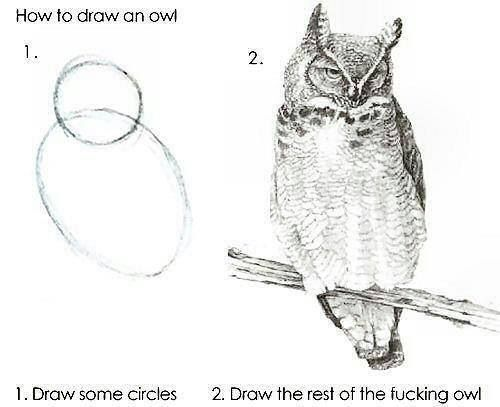
\includegraphics[width=8cm]{img/owl}
%\end{minipage}
%\end{textblock*}
%\end{frame}


%\begin{frame}{Ever heard of a 'comfort zone'?}
%\setstretch{1.2}
%\begin{textblock*}{\framewidth-0.8cm}(0.0cm,1.5cm) % {block width} (coords)
%\begin{itemize}
%  \item It's crucial to be out of it to learn something new
%  \item So I made this presentation in TeX
%\end{itemize}
%\end{textblock*}
%\end{frame}

%\begin{frame}{Fast-forward to 2016}
%\setstretch{1.2}
%\begin{textblock*}{\framewidth-0.8cm}(0.7cm,1.5cm) % {block width} (coords)
%Brendan Gregg declared Linux DTrace-complete!
%\begin{minipage}{\textwidth}
%  \centering
%  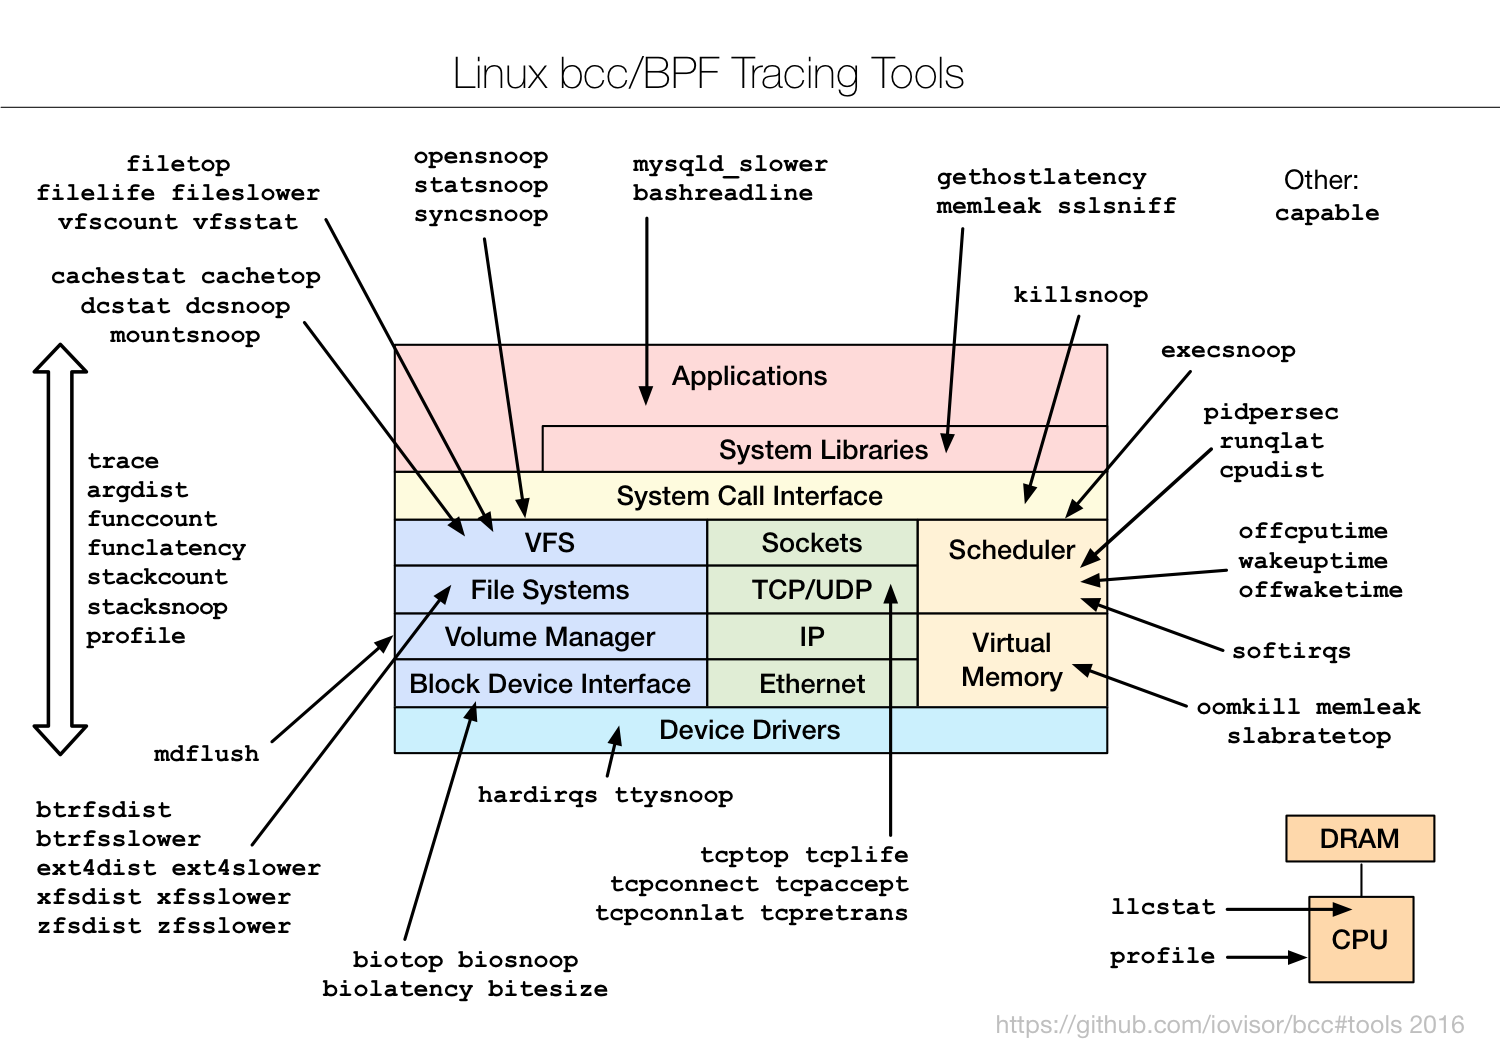
\includegraphics[height=6.6cm]{img/2016.png}
%\end{minipage}
%\end{textblock*}
%\end{frame}

\begin{frame}{\ \ \ Выводы}
\setstretch{1.2}
\begin{textblock*}{\framewidth-0.8cm}(0.5cm,1.5cm) % {block width} (coords)
\begin{itemize}
  \item TeX is great!
  \item Nim is great too!
  \item Flamegraphs are great!
  \item Linux is great!
  \item Death can be by {\TeX} too!
\end{itemize}
\end{textblock*}
\end{frame}

\begin{frame}{\ \ \ Вопросы, пожалуйста?}
\setstretch{1.2}
\begin{textblock*}{\framewidth-0.8cm}(0.5cm,1.5cm)
\begin{itemize}
  \item ...?
  \item ...?
  \item ...?
\end{itemize}
\end{textblock*}
\end{frame}

\begin{frame}{\ \ \ So long, and thanks for all the fish}
\setstretch{1.2}
\begin{textblock*}{\framewidth-0.8cm}(0.5cm,1.5cm)
\begin{itemize}
  \item \href{mailto:achistyakov@dataart.com}{\color{blue}{achistyakov@dataart.com}}
  \item \href{https://telegram.me/lhommequipleure}{\color{blue}{https://telegram.me/lhommequipleure}}
\end{itemize}
\end{textblock*}
\end{frame}
\end{Large}

\end{document}